\capitulo{6}{Trabajos relacionados}

%Este apartado sería parecido a un estado del arte de una tesis o tesina. En un trabajo final grado no parece obligada su presencia, aunque se puede dejar a juicio del tutor el incluir un pequeño resumen comentado de los trabajos y proyectos ya realizados en el campo del proyecto en curso.
\section{Activiti-Api}

Es una aplicación bastante parecida en funcionalidad. Se ha implementado como aplicación de escritorio en lenguaje Java. En algunos aspectos ha sido modelo para el desarrollo de este proyecto software. Esta alojado en GitHub\footnote{\url{https://github.com/dba0010/Activiti-Api}} y se puede obtener y ejecutar. Se muestra la ventana principal en la Fig. \ref{fig:M6_ActivitiApi_Ppal}.

\begin{figure}[h!]
	\centering
	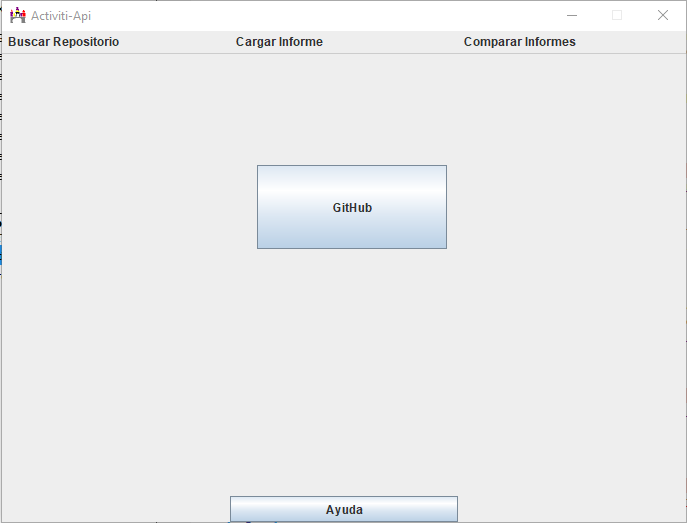
\includegraphics[width=0.65\textwidth]{M6_ActivitiApi_Ppal}
	\caption{Ventana principal de Activiti-Api}\label{fig:M6_ActivitiApi_Ppal}
\end{figure}

El aspecto que más llamó la atención para este proyecto es la forma de buscar repositorios. Permite establecer una conexión a GitHub iniciando sesión mediante usuario y contraseña o entrar en ``Modo desconectado'', como se muestra en la Fig. \ref{fig:M6_Comp_Conn}. En este proyecto se ha ampliado esta funcionalidad añadiendo más formas de conexión. Además, se ha diseñado un framework que facilita la extensibilidad hacia otras forjas de repositorios como GitHub o Bitbucket.

%\begin{figure}[!h]
%	\centering
%	\includegraphics[width=0.65\textwidth]{M6_ActivitiApi_Con}
%	\caption{Conexión a GitHub mediante Activiti-Api}\label{fig:M6_ActivitiApi_Con}
%\end{figure}

Una vez establecida la conexión permite elegir un proyecto para calcular sus métricas de evolución. Para ello hay que indicar un usuario, se cargará un desplegable con los proyectos de ese usuario y solo habría que escoger uno.

%\begin{figure}[!h]
%	\centering
%	\includegraphics[width=0.65\textwidth]{M6_ActivitiApi_Proyectos}
%	\caption{Selección de un proyecto para obtener las métericas en Activiti-Api}\label{fig:M6_ActivitiApi_Proyectos}
%\end{figure}

También se han tomado ideas de cómo calcular las métricas e implementar el framework de medición del que se habla en la sección \ref{sect:3_3_3_FrameworkMedicion} en el apartado ``Framework de medición''.

\subsection{Comparando este Evolution Metrics Gauge con Activiti-Api}

A continuación se muestran las diferencias entre `Evolution Metrics Gauge' y `Activiti-Api'.

\subsubsection{Interfaz}

En este proyecto se ha optado por implementar una aplicación Web en lugar de una aplicación de escritorio.

\subsubsection{Conexión}

Para obtener información de los proyectos, \textit{Activiti-Api} permite establecer una conexión a GitHub mientras que \textit{Evolution Metrics Gauge} permite establecer conexión a GitLab. Además, permite extender la funcionalidad a otras forjas de repositorios como GitHub.

\textit{Activiti-Api} permite dos tipos de conexión: iniciar sesión a GitHub mediante usuario y contraseña o ``Modo desconectado'' (establece una conexión pública). \textit{Evolution Metrics Gauge} permite iniciar sesión a GitLab mediante usuario y contraseña o por medio de un token de acceso personal, incluso permite establecer una conexión pública o directamente trabajar sin conexión sobre la aplicación. Dependiendo de la conexión escogida se limitará la funcionalidad de la aplicación. Por ejemplo, sin conexión no es posible añadir repositorios. Esta comparativa de las interfaces se puede ver en la Fig. \ref{fig:M6_Comp_Conn}.

En \textit{Evolution Metrics Gauge} se muestra al usuario de la aplicación el tipo de conexión escogida en todo momento (Ver Fig. \ref{fig:M6_Open_Conn_Info}) y la información de sesión iniciada en caso de que se haya iniciado sesión en GitLab, esta información no es visible en \textit{Activiti-Api}.

\begin{figure}[!h]
	\centering
	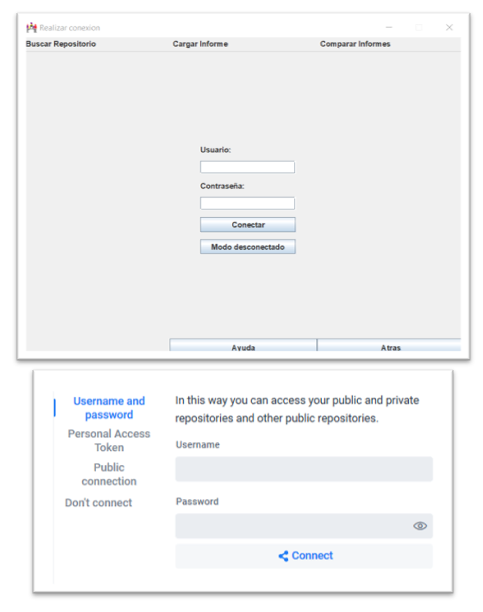
\includegraphics[width=0.75\textwidth]{M6_Comp_Conn}
	\caption{Comparación de las interfaces de conexión. Arriba `Activiti-Api', debajo `Comparador de métricas de evolución en repositorios software'}\label{fig:M6_Comp_Conn}
\end{figure}
\FloatBarrier

\begin{figure}[!h]
	\centering
	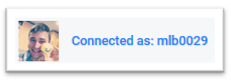
\includegraphics[width=0.4\textwidth]{M6_Open_Conn_Info}
	\caption{Visualización del tipo de conexión establecida}\label{fig:M6_Open_Conn_Info}
\end{figure}
\FloatBarrier

\subsubsection{Gestión de proyectos y evaluación de métricas}

\textit{Activiti-Api} permite evaluar un solo proyecto o comparar dos. La comparación se ha definido de forma estática durante el desarrollo del proyecto, permaneciendo invariable en tiempo de ejecución.

\textit{Evolution Metrics Gauge} permite añadir múltiples proyectos, evaluarlos y compararlos mediante el cálculo estadístico de cuartiles para hallar los valores umbrales de cada métrica. Por tanto la comparación puede ser dinámica a partir de los proyectos que se escojan para la comparativa, aunque también se han definido unos valores umbrales predefinidos a partir de unas estadísticas obtenidas de un conjunto de datos obtenidos a partir de TFGs y publicado en GitHub \footnote{\url{https://github.com/clopezno/clopezno.github.io/blob/master/agile_practices_experiment/DataSet_EvolutionSoftwareMetrics_FYP.csv}}. Además, permite gestionar perfiles de métricas con diferentes umbrales para distintos contextos de aplicación.

\textit{Activiti-Api} genera un informe con los resultados de las métricas de un proyecto, varios gráficos y permite generar un informe de comparativa entre dos proyectos (ver Fig. \ref{fig:M6_AA_Comparativa}). \textit{Evolution Metrics Gauge} muestra los resultados de varios proyectos en forma de tabla (ver Fig. \ref{fig:M6_EMC_Comparativa}).

\begin{figure}[!h]
	\centering
	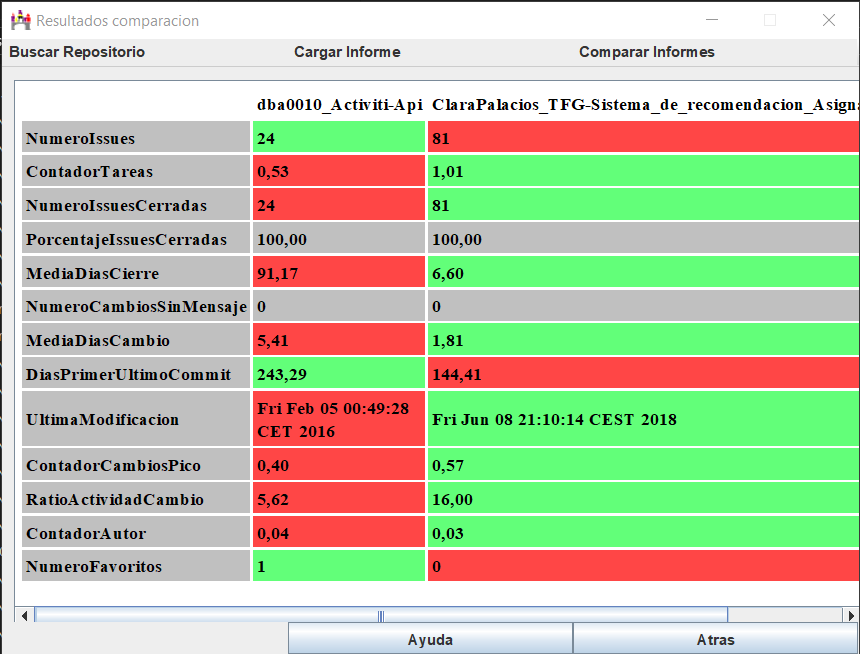
\includegraphics[width=0.65\textwidth]{M6_AA_Comparativa}
	\caption{Comparación de dos proyectos utilizando Activiti-Api}\label{fig:M6_AA_Comparativa}
\end{figure}
\FloatBarrier

\begin{figure}[!h]
	\centering
	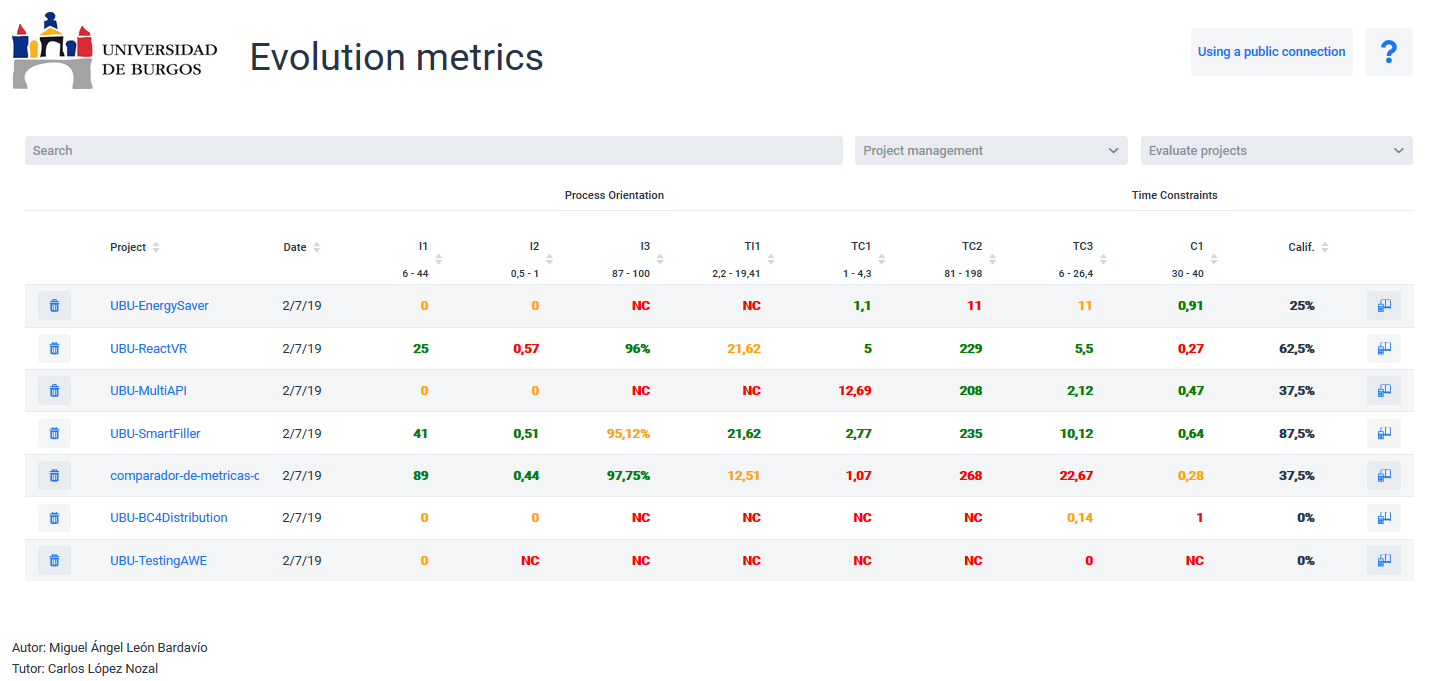
\includegraphics[width=0.90\textwidth]{M6_EMC_Comparativa}
	\caption{Comparación de varios proyectos utilizando Evolution metrics comparison}\label{fig:M6_EMC_Comparativa}
\end{figure}
\FloatBarrier

%\todo Nombre corto de la app: Evolution metrics o Evolution Metrics Comparison

\subsubsection{Mantenibilidad y extensibilidad}

\textit{Evolution Metrics Gauge} ha preparado un framework para poder extenderse a otras forjas de repositorios. Ha sido implementado para obtener datos desde GitLab, pero es fácilmente extensible a otras forjas como GitHub. \textit{Activiti-Api} no permite esta extensibilidad e incluye demasiadas dependencias con GitHub API.

Ambos proyectos siguen la solución basada en frameworks propuesta en \textit{Soporte de Métricas con Independencia del Lenguaje para la Inferencia de Refactorizaciones} \citep{marticorena_sanchez_soporte_2005}. El objetivo del \textit{framework} es la reutilización en la implementación del cálculo de métricas. De hecho, \textit{Activiti-Api} ha servido de ejemplo para la implementación del motor de métricas de este trabajo.

\section{Otros trabajos relacionados}
\begin{itemize}
	\item \textbf{Soporte de Métricas con Independencia del Lenguaje para la Inferencia de Refactorizaciones}. En él, se ha basado la construcción del subsistema ``motor de métricas'', como se puede ver en la sección \ref{sect:3_3_3_FrameworkMedicion} en el apartado `Framework de medición'.
	
	\item \textbf{Software Project Assessment in the Course of Evolution -  Jacek Ratzinger}. Es de este trabajo de donde se han obtenido las métricas de control con las que trabaja \textit{Evolution Metrics Gauge}. Hay una explicación detallada en el apartado \ref{sect:3_3_2_MetricasControl} en el apartado `Métricas de control: medición de la evolución o proceso de software'.
\end{itemize}

